\pgfdeclarelayer{background}
\pgfdeclarelayer{foreground}
\pgfsetlayers{background,main,foreground}

% Define a few styles and constants
\tikzstyle{l1}=[draw, fill=black!15, text width=4em, 
    text centered, minimum height=3em, rounded corners]
\tikzstyle{l2} = [l1, text width=6em, fill=black!15, 
    minimum height=10em, rounded corners]
\tikzstyle{ann} = [above, text width=5em]
\def\blockdist{3.3}
\def\edgedist{1.5}
\def\minedgedist{1.0}
\def\lowlev{0.25}
\def\midlev{0.45}
\def\toplev{0.5}

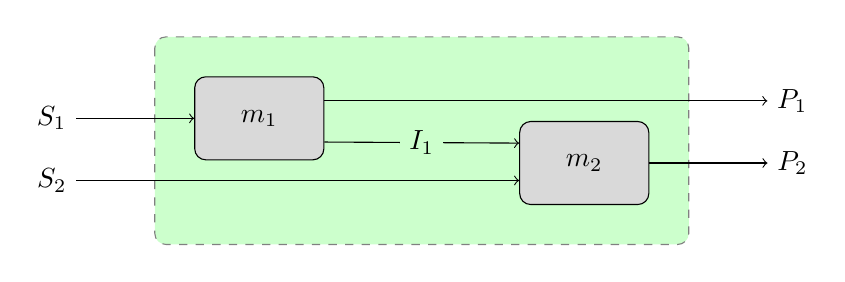
\begin{tikzpicture}
	%uncomment to show a dot at the center
	%\filldraw [red] (0,0) circle (5pt);
	
	\node (m2) [l1] {$m_2$};
    
    %\path (m3.150)+(-\blockdist,0.09) node (m2) [l1] {$m_2$};
    \path (m2.150)+(-\blockdist,0.09) node (m1) [l1] {$m_1$};
            
    \path [draw, ->] (m1.-20) -- node [fill=green!20] {$I_1$} (m2.163) ;
%     \path [draw, ->] (m2.-15) -- node [below] {$I_2$} 
%         (m3.165) ;
        
%     \path (m3.south west)+(-0.6,-0.4) node (l1b) {};
    %3.72*\edgedist
    \draw [->] (m1.15) -- +(3.75*\edgedist,0) node [right] {$P_1$};
    \draw [->] (m2.0) -- +(\edgedist,0) node [right] {$P_2$};
%    	\draw [->] (m3.15) -- +(\edgedist,0) node [right] {$P_3$};
%     \draw [->] (m3.-15) -- +(\edgedist,0) node [right] {$P_4$};
   	    
    \draw [->] (m1.180)+(-\edgedist,0) node[left] {$S_1$} -- (m1.180);
    %\draw [->] (m1.195)+(-\edgedist,0) node[left] {$S_2$} -- (m1.195);
%     \draw [->] (m3.195)+(-6.44*\edgedist,0) node[left] {$S_3$} -- (m3.195);
\draw [->] (m2.195)+(-3.75*\edgedist,0) node[left] {$S_2$} -- (m2.195);             
    \begin{pgfonlayer}{background}
        % Compute a few helper coordinates
        \path (m1.west |- m1.north)+(-\toplev,\toplev) node (a) {};
        \path (m2.south -| m2.east)+(\toplev,-\toplev) node (b) {};
        \path[fill=green!20,rounded corners, draw=black!50, dashed]
            (a) rectangle (b);
%         \path (m1.north west)+(-\midlev,\midlev) node (a) {};
%         \path (m2.south -| m2.east)+(\midlev,-\midlev) node (b) {};
%         \path[fill=green!20,rounded corners, draw=black!50, dashed]
%             (a) rectangle (b);
% 		\path (m2.north west)+(-\midlev,0.3) node (a) {};       
% 		\path (m3.south east)+(\midlev,-\midlev) node (b) {};       
%   		\path[fill=red!20,rounded corners, draw=black!50, dashed]
%             (a) rectangle (b);
% 		\path (m3.north west)+(-\lowlev,\lowlev) node (a) {};
% 		\path (m3.south east)+(\lowlev,-\lowlev) node (b) {};       
%   		\path[fill=green!20,rounded corners, draw=black!50, dashed]
%             (a) rectangle (b);
% 		\path (m1.north west)+(-\lowlev,\lowlev) node (a) {};
% 		\path (m1.south east)+(\lowlev,-\lowlev) node (b) {};       
%   		\path[fill=red!20,rounded corners, draw=black!50, dashed]
%             (a) rectangle (b);
    \end{pgfonlayer}
\end{tikzpicture}